\section{15.10.2025}{um}

Co jest dziedziną funkcji holomorficznej?
\begin{enumerate}
  \item $U\subseteq \C$ otwarty
  \item $U\subseteq \overline{C}$ otwarty
\end{enumerate}
chcemy wyjść poza te możliwości i zadać konkretniejsze pytanie: co jest dziedziną funkcji $\sqrt{z}$?
\begin{enumerate}
  \item "dwuwartościowa funkcja homolorficzna na $\C^\times=\C\setminus\{0\}$"
  \item weźmy dwie kopie $\C^\times$ i próbujemy na tym określać peirwiastek z $z$.

    na górnej kopii zaczynamy w $1$ i idziemy do $1$, a na dolnej do $-1$

    \begin{center}
      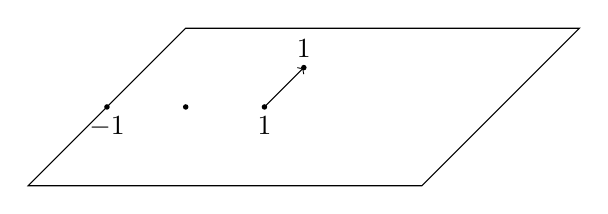
\begin{tikzpicture}
        \draw (0,0) -- (5, 0)--(7, 2)--(2, 2) -- cycle;
      \fill (2, 1) circle (1pt);
      \fill (3, 1) circle (1pt) node [below] {$1$};
      \fill (1, 1) circle (1pt) node [below] {$-1$};
      \fill (3.5, 1.5) circle (1pt) node [above] {$1$};
      \draw[->] (3, 1) -- (3.5, 1.5); 
      \end{tikzpicture}
    \end{center}
    Riemann proponuje pomysł naprawy: rozetnijmy te kopie $\C^\times$ wzdłuż $\R_-$
    \begin{center}
      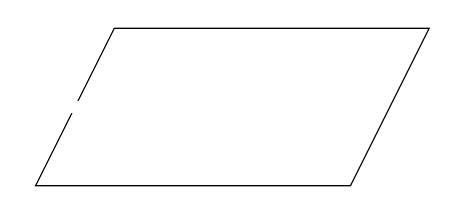
\begin{tikzpicture}
        \draw (0,0) -- (4, 0) -- (5, 2) -- (1, 2) -- cycle;
        \fill[white] (-.1, .9) -- (2.5, 1) -- (-.1, 1.1) -- cycle;
      \end{tikzpicture}
    \end{center}
    teraz sklejamy "na krzyż" rozcięcia" i dostajemy tzw. powierzchnię Riemanna pierwiastka $\sqrt{z}$, która dwukrotnie nakrywa $\C^\times$.

    Na tej powierzchni $\sqrt{z}$ jest jednoznaczną funkcją holomorficzną.
\end{enumerate}

\begin{fact}{}{}
  Niech $p:\C^2\to\C^2$ będzie holomorficzną funkcją dwóch zmiennych. Niech $\Sigma=\{(x,y)\in\C^2\;:\;p(x,y)=0\}$. Załóżmy, że dla wszystkich $(x_0, y_0)\in\Sigma$ któraś z pochodnych cząstowcyh jest niezerowa $p_x(x_0, y_0)\neq 0$ lub $p_y(x_0, y_0)\neq 0$.

  Wtedy w otoczeniu każdego $(x_0, y_0)\in\Sigma$ jest wykresem funkcji holomorficznej, tzn. istnieje $D_1\times D_2\in (x_0, y_0)$ takie, że 
  $$\Sigma\cap (D_1\times D_2)=\{(x, f(x))\;:\;x\in D_1\},$$
  $f:D_1\to D_2$ holo $(p_y\neq 0)$ lub 
  $$\Sigma\cap (D_1\times D_2)=\{(g(y), y)\;:\;y\in D_2\},$$
  $g:S_2\to D_1$ holo $(p_x\neq 0)$
\end{fact}

\begin{proof}
  Załóżmy, że $p_y(x_0, y_0)\neq 0$. Chcemy popatrzeć na pionową prostą $x=x_0$. Po ograniczeniu do niej funkcja jest holomorficzna, która się zeruje w $y_0$, ale niezeruje się w małym dyszczku $D_2$ o środku w $(x_0, y_0)$ poza samym punktem $(x_0, y_0)$.

  Wtedy
  $$\frac{1}{2\pi i}\int_{\partial D_2} \frac{p_x(x_0 ,y)}{p(x_0, y)} dy=1$$
  możemy temu pysiowi machać $x_0$, czyli przesuwać płaszczyznę $x=x_0$ i całkować po analogicznym okręgu $\partial D_2$. $p$ jest niezerowa na otoczeniu $\{x_0\}\times\partial D_2$, np. $D_1\times\partial D_2$.

  {\color{red}tutaj rysuneczki}

  Dla $x\in D_1$ mamy
  $$\frac{1}{2\pi i}\int_{\partial D_2}\frac{p_y(x,y)}{p(x,y)}dy=1$$
  całka w ciągły sposób zależy od $x$, dla $x=x_0$ była równa jeden więc na całości też jest równa jeden.

  To znaczy, że w $\{x\}\times D_2$ funkcja $p$ ma jedno zero, które można zapisać wzorem
  $$f(x)=\frac{1}{2\pi i}\int_{\partial D_2}\frac{yp_y(x,y)}{p(x,y)}dy$$
\end{proof}

W sytuacji z faktu: kiedy $F:\Sigma\to \C$ uznamy za holomorficzną?

  $F$ holomorficzna w $\Sigma$ gdy holomorficzna w otoczeniu każdego $(x_0, y_0)\in\Sigma$, czyli jeśli $x\mapsto F(x, f(x))$ (lub drugi wariant) jest holomorficzna w otoczeniu w $x_0$ lub $y_0$
  
jeśli $p_x(x_0, y_0)\neq 0\neq p_y(x_0, y_0)$ to nie ma sprzeczności.

KOLEJNY OBRAZEK

$f$ i $g$ są holomorficzne, więc definicja jest poprawna :p - to jest komentarz do obrazka btw

\begin{definition}{}{}
  Powierzchnią Riemanna $\Sigma$ nazywamy topologiczną przestrzeń Hausdorffa wyposażoną w rodzinę map $(U_\alpha, \phi_\alpha)$ taką, że 
  \begin{enumerate}
    \item $\bigcup U_\alpha=\Sigma$
    \item $U_\alpha$ otwarte
    \item $\phi_\alpha:U_\alpha\to V\subseteq \C$ homeomorfizm na otwarty podzbiór $\C$
    \item $\phi_\alpha\circ\phi_\beta^{-1}$ jest holomorifczne tam gdzie jest określone
  \end{enumerate}
\end{definition}

\begin{conclusion}{}{}
  $\Sigma$ jak w fakcie wcześniej jest powierzchnią Riemanna.
\end{conclusion}

\begin{definition}{}{}
  $\Sigma$ - powierzchnia Riemanna, $f:U\to \C$ ($U\subseteq\Sigma$ otwarty). Mówimy, że $f$ jest holomorficzna ($f\in O(U)$) jeśli każda $f\circ\phi_\alpha^{-1}$ jest holomorficzna na swojej dziedzinie.

  Wariant dla dwóch powierzchni Riemanna.
\end{definition}

\begin{example}[m]
\item $\Sigma=Z(y^2-x)$ zera tego wielomianu

  KOLEJNY RYSUNEEEEEEEEEEEEEEEEEK
  
  zbiór rozwiązań równania $y^2=p(x)$ nazywa się czasem powierzchnią hipereliptyczną
\end{example}

\subsection{Ilorazy}

$\C/\Z[i]$ - no ze to torus jest

mapki: dla $z\in\C$ wybieramy $V_z=B(z, \frac{1}{2})$

Odwzorowanie ilorazowe przekształca $V_z$ holomorficznie na $U_z\subseteq \C/\Z[i]$

odwrotności takich odwzorowań przyjmujemy za mapy

odwzorowania między mapami to po  prostu przesunięcia, więc śmiga

jeśli $z_1, z_2\in\C$ liniowo niezależna nad $\R$ to definiujemy kratę $\Lambda=\Z z_1+\Z z_2$ i wtedy iloraz $\C/\Lambda$ też jest powierzchiną Riemanna.

niezależnie od wyboru kraty $\Lambda$, iloraz zawsze jest homeomorficzny z torusikiem

jednak nie zawsze $\C/\Lambda_1$ i $\C/\Lambda_2$ są holomorficzne (struktury zespolone mogą się nie zgadzać)

\begin{center}
  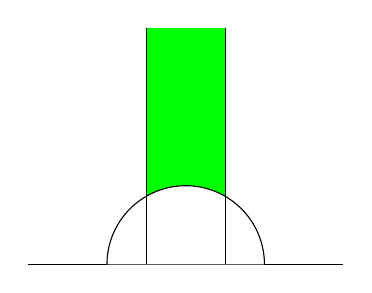
\begin{tikzpicture}
    \draw (-2, 0)--(2, 0);
    \fill[green] (-.5, 0)--(.5, 0)--(.5, 3)--(-.5, 3);
    \fill[white] (1, 0) arc (0:180:1);
    \draw (1, 0) arc (0:180:1);
    \draw (-.5, 0)--(-.5, 3);
    \draw (.5, 0)--(.5, 3);
  \end{tikzpicture}
\end{center}
zielony obszar nazywam $M$, $M\ni \tau\mapsto \C/\Z-1+\Z\tau$

$\tau$ parametryzuje możliwe struktury holomorficzne na torusiku

Na przykład $y^2=x(x-1)(x-2)(x-3)$ bierzemy dwie płaszczyzny, rozcinamy między $0$ a $1$ i między $2$ a $3$ i sklejamy na krzyż, ale to można sobie wyobrażać jako dwie płaszczyzne połączone dwoma tubkami (skręconymi, które można odkręcić)

jak uzwarcimy te dwie płaszczyzny to dostajemy torus

GENERALNIE TUTAJ JEST OBRAZEK

pytanie: czy da się podobnie badać powierzchnie Riemanna jako ilorazy dysku?

kiełki i kontynuacja analityczna

\begin{definition}{}{}
  \begin{enumerate}
    \item niech $z_0\in\C$ na parach $(U, f)$, gdzie $z_0\in U\subseteq \C$ otwarty, $f\in O(U)$, wprowadzamy relację równoważności $\sim_{z_0}$ $(U,f)\sim_{z_0}(V, g)$ $\iff$ istnieje otwarty $z_0\in W\subseteq U\cap V$ taki, że $f|_W=g|_W$

      klasy równoważności tego cuda to kiełki (oznaczamy $\underline{f}_{z_0}$ klasę $(U, f)$ pod relacją $\sim_{z_0}$) 
    \item $O_\C$ - przestrzeń wszystkich kiełków funkcji holomorficznych

      na nim chcemy określić pewną topologię

      dla $(U, f)$ podzbiór $O_\C$: 
      $$O(U, f)=\{\underline{f}_z\;:\;z\in U\}$$
      jest otwarty (baza topologii)

      to jest Hausdorffa
    
      rzut $O_\C\ni \underline{f}_z\mapsto z\in\C$ jest lokalnym homeomorfizmem
    \item dla $f\in O(U)$ składowa spójna $O_\C$ zawierająca $O(U,f)$ to z definicji powierzchnia Riemanna funkcji $f$
  \end{enumerate}
\end{definition}

$\C P^2$

$p(x,y)=0$ wielomian to mamy zera tego wielomianu

$\C^2\subseteq \C P^2=\{l\;:\;l<\C^3,\;\dim_\C(l)=1\}=\{[x:y:z]\}$ nie chce mi się pisać porządnie

trzy różne sposoby włożeni a$\C^2$

to robienie że wielomian ma każdą zmienną w tym samym stopniu





